Wolfenstein 3D was not the first FPS the team produced. Back when they worked at Softdisk, they worked on two games: Hovertank 3D and Catacomb 3D.\\
\par
\section{Hovertank 3D}
Howertank 3D (a.k.a Hovertank, Hovertank 3-D or Hovertank One)  is a vehicular combat game published by Softdisk in April, 1991. John Carmack's research in the game's engine took six weeks, two weeks longer than any engine he wrote before it. The game has no music and suffered from its 16 colors EGA technology.
\begin{figure}[H]
\centering
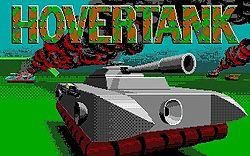
\includegraphics[width=\textwidth]{screenshots/Hovertank_3D_title_screen.png}
\end{figure}

\begin{figure}[H]
\centering
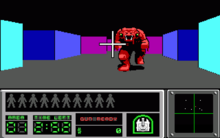
\includegraphics[width=\textwidth]{screenshots/Hovertank_3D_screen.png}
\end{figure}



\section{Catacomb 3D}
Upon completion of Hovertank, the team of four improved the engine with texture mapping for the wall. Also in EGA the graphism were much better. The rythm was slow and I would not call it a FPS. 
\begin{figure}[H]
\centering
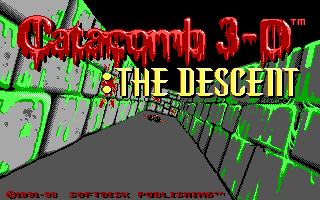
\includegraphics[width=\textwidth]{screenshots/Catacomb_3-D_The_Descent_title_screen.png}
\end{figure}

Fun to be able to destroy walls to discover secret sections. Fireballs.

\begin{figure}[H]
\centering
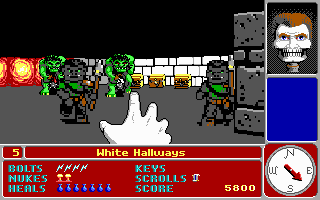
\includegraphics[width=\textwidth]{screenshots/Catacomb_3-D_The_Descent_screenshot.png}
\end{figure}

EGA based. Slower. Destroyable walls. Fun you could probe secret wall by just firing fireballs at them.



